\documentclass{beamer}
%Information to be included in the title page:
\title{Sample title}
\author{Anonymous}
\institute{Overleaf}
\date{2021}

\begin{document}

\frame{\titlepage}

\begin{frame}
\frametitle{Introduction}
\framesubtitle{Definitions}

\begin{itemize}
    \item \textbf{Options} are contracts that give \textbf{the holders} the right to buy/sell an \textbf{underlying asset} at a pre-established at some point in the future before or at the expiration date.
    
    \item The \textbf{strike} price is the pre-established price at which the holder will buy/sell the \textbf{option}.

    \item The \textbf{maturity} date is the expiration date of the contract.

    \item \textbf{Exercising} the option refers to the act of buying/selling the underlying asset.

    \item The \textbf{premium} is the money charged by the writer to the holder for entering the contract.
\end{itemize}

\end{frame}

\begin{frame}
    \frametitle{Introduction}
    \framesubtitle{Definitions}
    
    \begin{itemize}
        \item \textbf{Options} are contracts that give \textbf{the holders} the right to buy/sell an \textbf{underlying asset} at a pre-established at some point in the future before or at the expiration date.
        
        \item The \textbf{strike} price is the pre-established price at which the holder will buy/sell the \textbf{option}.
    
        \item The \textbf{maturity} date is the expiration date of the contract.
    
        \item \textbf{Exercising} the option refers to the act of buying/selling the underlying asset.
    
        \item The \textbf{premium} is the money charged by the writer to the holder for entering the contract.
    \end{itemize}
    
\end{frame}

\begin{frame}
\frametitle{American options pricing problem}
\framesubtitle{Definitions}
\centering
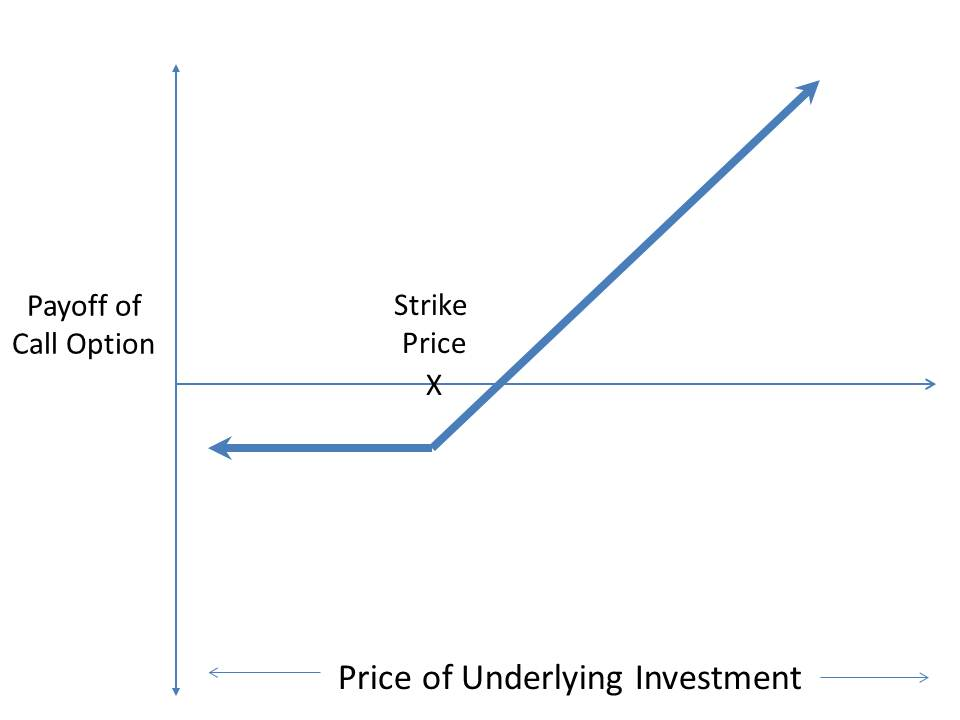
\includegraphics[width=.9\textwidth]{images/Call_Option}

\end{frame}

\begin{frame}
    \frametitle{American options pricing problem}
    \framesubtitle{Definitions}
    \centering
    \begin{tabular}{ |c|c|c| }
        \hline
            & At time maturity & Before and at maturity \\ \hline
        Buy & European call options & American call options \\  \hline
        Sell & European put options & American put options \\ \hline
    \end{tabular}
\end{frame} 

\begin{frame}
    \frametitle{American options pricing problem}
    \framesubtitle{Definitions}
    \textbf{Goal:}
    Given an American call/put option with a \textbf{strike price} ($K$), 
    and \textbf{maturity date} ($T$), find the \textbf{premium} ($V(S)$) charged 
    by the \textbf{ writer} to the holder such as there is no \textbf{arbitrage} 
    opportunity.

    Arbitrage refers to the possibility that either the writer or holder to make a risk-free profit. 
\end{frame}

\begin{frame}
    \frametitle{American options pricing problem}
    \framesubtitle{Mathematical model}
    \begin{itemize}
        \item $\mathcal{T}: [0, T]$
        \item $\mathcal{X}: [0, \infty)$
        \item $\mathcal{D}: \mathcal{X}\times\mathcal{T}$
        \item $V: \mathcal{D} \rightarrow \mathbb{R}$
    \end{itemize}
\end{frame}

\begin{frame}
    \frametitle{American options pricing problem}
    \framesubtitle{Mathematical model}
    The payoff of function is defined as

    \begin{subequations}
        \begin{equation}
            H(S, t) = \max(S - K, 0)
        \end{equation}
        \begin{equation}
            H(S, t) = \max(K-S, 0)
        \end{equation}
    \end{subequations}
\end{frame}

\begin{frame}
    \frametitle{American options pricing problem}
    \framesubtitle{Black-Scholes model}
    \begin{itemize}
        \item American options is bounded from below by the payoff $V(S, t) \ge H(S, t)$
        \item $\mathcal{D}$ is divided in two exclusive regions: the exercise region $\mathcal{S}$ and continuation region $\mathcal{C}$. 
        \item $\bar{S}(t)$ is the optimal exercise price.
        \item The price $V(S, t)$ behaves similar to the price of a European option in the continuation region.
        \item $\mathcal{S}: \{(S,t): V(S, t) = H(S, t)\}$
        \item $\mathcal{C}: \{(S,t): V(S, t) > H(S, t)\}$
        \item $\partial{\mathcal{C}}: \{(S,t): \bar{S}(t) = S\}$
    \end{itemize}
\end{frame}

\begin{frame}
    \frametitle{American options pricing problem}
    \framesubtitle{Free boundary problem}

    \begin{equation}
        \begin{cases}
            \dfrac{\partial{V}}{\partial{t}} + \dfrac{1}{2}\sigma^2\dfrac{\partial^2{V}}{\partial{S^2}} + (r-\delta)\dfrac{\partial{V}}{\partial{S}} - rV = 0 & \text{for $(S, t) \in \mathcal{C}$} \\
            V(S, t) = H(S, t) & \text{for $(S, t) \in \partial{\mathcal{C}}$}
        \end{cases}
    \end{equation}
\end{frame}

\begin{frame}
    \frametitle{American options pricing problem}
    \framesubtitle{Free boundary problem}


\end{frame}

\end{document}